\documentclass[10pt,draftclsnofoot,onecolumn,compsoc]{IEEEtran}
\usepackage[letterpaper, portrait, margin=0.75in]{geometry}
%\usepackage[myheadings]{fullpage}
\usepackage{fancyhdr}
\usepackage{lastpage}
\usepackage{graphicx,  subcaption,  booktabs}
\usepackage[T1]{fontenc}
\usepackage[font=small, labelfont=bf]{caption}
%\usepackage{fourier}
\usepackage[protrusion=true, expansion=true]{microtype}
\usepackage[english]{babel}
%\usepackage{sectsty}
\usepackage{url, lipsum}
\usepackage{tikz}
\usepackage[section]{placeins}
\usepackage{makeidx}
\newcommand{\subparagraph}{}
\usepackage{titlesec}
\usepackage{enumitem}

\makeatletter
\renewcommand{\@IEEEsectpunct}{ \\ \\ \,}% Modified from {:\ \,}
\makeatother

\setlength{\parindent}{0em}
\setlength{\parskip}{1em}
\renewcommand\thesection{\arabic{section}}
\renewcommand\thesubsection{\thesection.\arabic{subsection}}
\renewcommand\thesubsubsection{\thesubsection.\arabic{subsubsection}}

\makeatletter
\renewcommand\paragraph{\@startsection{paragraph}{4}{\z@}%
                                    {0ex \@plus0ex \@minus.0ex}%
                                    {0em}%
                                    {\normalfont\normalsize\bfseries}}
\makeatother

\renewcommand\thesectiondis{\arabic{section}}
\renewcommand\thesubsectiondis{\thesectiondis.\arabic{subsection}}
\renewcommand\thesubsubsectiondis{\thesubsectiondis.\arabic{subsubsection}}


\titleformat{\section}
       {\normalfont\fontfamily{phv}\fontsize{14}{17}\bfseries}{\thesection}{1em}{}
\titleformat{\subsection}
       {\normalfont\fontfamily{phv}\fontsize{14}{17}\bfseries}{\thesubsection}{1em}{}
\titleformat{\subsubsection}
       {\normalfont\fontfamily{phv}\fontsize{14}{17}\bfseries}{\thesubsubsection}{1em}{}


\newcommand{\namesigdatehrule}[1]{\par\tikz \draw [blue, densely dotted, ultra thick] (0,0) -- (#1,0);\par}
\newcommand{\namesigdate}[2][5cm]{%
\begin{minipage}{#1}%
    #2 \vspace{0.8cm}\namesigdatehrule{#1}\smallskip
    \small \noindent\textit{Signature}
    \vspace{0.8cm}\namesigdatehrule{#1}\smallskip
    \small \textit{Date}
\end{minipage}
}


\newcommand{\HRule}[1]{\rule{\linewidth}{#1}}
\newcommand*\tick{\textsc{\char13}}
\linespread{1}
\setcounter{tocdepth}{5}
\setcounter{secnumdepth}{5}

\makeindex

\begin{document}
%\title{HyRo (Working title)}
%\author{Jason Klindtworth  |  Josh Asher  |   Layne Nolli}
%\date{}
%\maketitle
\begin{titlepage}
	\centering
	{\scshape\LARGE HyRo \par}
	%\vspace{1cm}
	{\scshape\LARGE Team 28\par}
	\vspace{1cm}
	{\scshape\Large Jason Klindtworth  |  Josh Asher  |   Layne Nolli}
	\noindent\makebox[\linewidth]{\rule{17cm}{2pt}}
	\vspace{1cm}
	{\huge\bfseries CS461\par}
	\vspace{2cm}
	{\Large\itshape Fall 2016\par}
	\vspace{4cm}
	{\large Software Design Document\par}\vspace{2cm}
	{\large Abstract\par}
	\vspace{1cm}
	High Altitude rockets have a distinct advantage in using Hybrid propulsion systems. These systems are complex and present challenges in remote telemetry including launch initialization and controlling remote fuel filling/disconnect. High altitude rockets also contain an array of sensors that collect data which needs to be visualized in a human friendly format. The goal of HyRo is to provide mechanisms for remotely launching and controlling the fuel systems on a hybrid propulsion system through onboard embedded circuitry/software that communicates to launch team via radio waves. This circuitry/software will also communicate sensor data to the ground. Sensor data is displayed in our visualization software in an appealing, human readable way. \par

	\noindent\makebox[\linewidth]{\rule{17cm}{2pt}}
	\vfill

% Bottom of the page
	{\large \today\par}
\end{titlepage}

%\newpage
%\sectionfont{\scshape}
%\title{Abstract}

\setcounter{tocdepth}{2}
\tableofcontents
\newpage

\section{Introduction}
\subsection{Scope}
This Design Document described in detail both the structure and the components of the HyRo deployment software interface and database. It also includes the implementation details required to accurately and completely incorporate the specific requirements associated with this project as detailed in the Requirements Document. Because of the contents of this document, it is assumed that the reader has familiarized themselves with the projects Requirements Document and is aware of the specific needs of this software package and graphical user interface. There is also an assumed general knowledge of computer programing knowledge as this document will rely heavily on the explanation of specific software functions and processes that will be designed in order to accomplish all of the needed requirements for this project. 
\subsection{Purpose}
This Design Document serves the following purposes:
\begin{itemize}
	\item To fully describe the structure, functions, data, and algorithms which will be implemented in the software package.
	\item To point out and identify both specific and general system resources that will be utilized.
	\item To assist the HyRo team in the production and implementation of test cases.
	\item To be used in order to verify full compliance with the requirements of the project.
	\item To aid the team in the general overview of the software package and what the capabilities are.
\end{itemize}
\subsection{Intended Audience}
The majority of the document is written for the benefit of knowledgeable software development and design professionals in order to gain specific knowledge of the HyRo software system and its intended capabilities. The intended audience for this documents is the HyRo team, including the following:
\begin{itemize}
	\item The project supervisor 
	\item The computer science sub-team working on the software package itself.
	\item The electrical engineering sub-team working on the hardware in which the software package will be incorporated into.
	\item the mechanical engineering sub-team working on the mechanical operations of the rocket which the software package will control or manipulate.
	\item Any related sub-team for the project that requires knowledge of the computer system or interface system for the rocket.
\end{itemize}
\subsection{Definitions}
\begin{description}
	\item[Hybrid Rocket] A rocket with an engine that uses both solid and liquid fuel.
	\item[I/O] Input and Output.
	\item[PWM] Pulse Width Modulation is used to control signal level on a electrical wire.
	\item[Beagle Bone Black] A miniature computer that will be used on-board our hybrid rocket to house our software.
	\item[Python Dictionary] A associative array accessed by key value pairs.
	\item[Oxidizer] Liquid gas used to accelerate the burning of solid fuel.
	\item[Accelerometer] Measures acceleration.
	\item[Gyroscope] Measure tilt relative to the earth.
	\item[Magnetometer] Measures the electric field around it.
	\item[Multi Threaded] A program that runs multiple methods in parallel to the main program allowing components to run independently.
	\item[Mutex Lock] Used to lock control of an area of memory while an operation is completed. If any other parts of the system attempt to access this part of memory while the lock is in place they will not be allowed to.
	\item[Boolean] A way to represent a true or false value in software.
\end{description}
\subsection{References}
\subsection{Overview}
\section{Design Considerations}
\section{System Architecture On-board the Rocket }	
The SDD module design of the software on-board the hybrid rocket detailed here after will explain the approach, methods, and properties of this component of the system. Software running on-board the rocket will communicate to software running on a traditional computer through a radio transceiver connected to the Beagle Bone Black. For convenience a diagram is provided below to show the entirety of the entire system. This section will  only cover the design of the software running on the Beagle Bone Black.
\subsection{Components} 
This section is intended to explain the components of the rocket we will be receiving and/or sending data too. It is a general overview of what could be part of the system as the rocket has not yet been designed. Exact sensors are not presented because they have not be chosen yet. Though collection of data from them will be the same regardless. This allows for easy expansion of sensors in the code if time allows.\par
At the moment we know the rocket will have an accelerometer, barometric/temperature sensor, and a servo to control filling, arming, and launching of the rocket. The sensors will be polled for data every 500 milliseconds and this data will be held in a buffer to be transmitted. Each sensor/servo has drivers built in python that will be used to access the sensors/servo data and in case of the servo sen PWM signals to control the movement of the servo.\par
The sensors and servo are connected to the Beagle Bone Black physically through I/O lines available on the board. The drivers define these connections and the functions to preform communication. There is a chance that the rocket design will change and we will need to create our own drivers for the new components. If that happens the driver design will be detailed under this section. At the moment all components used last year currently have drivers available.\par
\subsection{Data Format}
There are two buffers in this program. One to hold the sensor data and one to hold commands received. They are both globally available to the entire program.
\subsubsection{Sensor Data Buffer}
The sensor data buffer will be a python dictionary with keys relating to the name of the sensor output. For examples the temperature data will be stored in and accessed by the field "temperature".  The timestamps field is important to the radio transceiver polling function (detailed below) as this is what it uses to decided if the data is new. Some of these data items are not planned on being used by the ground software, but are included for future data visualization expansion.
\begin{description}
	\item[Buffer Name] dataBuffer
	\item[Buffer Keys]  -
		\begin{description}
			\item[time\_stamp] Time the current data was written to this buffer.
			\item[altitude] The altitude above ground level reading from the altitude sensor.
			\item[temp] The temperature reading from the temperature sensor.
			\item[a\_x] Accelerometer data from x axis.
			\item[a\_y] Accelerometer data from y axis.
			\item[a\_z] Accelerometer data from z axis.
			\item[g\_x] Gyroscope data from the x axis.
			\item[g\_y] Gyroscope data from the y axis.
			\item[g\_z] Gyroscope data from the z axis.
			\item[m\_x] Magnetometer data from the x axis.
			\item[m\_y] Magnetometer data from the x axis.
			\item[m\_z] Magnetometer data from the x axis.
			\item[tank\_pres] The pressure of the oxidizer tank.
			\item[chamber\_pres] The pressure of the combustion chamber
		\end{description}
\end{description}

\subsubsection{Command Buffer}
The command buffer will be used to store commands received from the traditional computer software component to be accessed by the command thread. A python list data structure will be used to provide easy pushing and popping of values. When a command is detected it is added to this array and as it is processed it is removed from the array.\par
{\bf Buffer Name:} commandBuffer \\
{\bf Example:}\\
commandBuffer = {} // empty \\
New command Received = arm add to buffer \\
commandBuffer = {0 : 'arm'} \\
New command Received = disarm add to buffer \\
commandBuffer = {0 : 'arm', 1:  'disarm'} \\
Command Processed = 'arm' \\
commandBuffer = { 0 :'disarm'} \\
Command Processed = 'disarm' \\
commandBuffer = {} //empty \\

 
\subsection{Methods and Threads}
This component will be designed in using multi threaded approach with helper functions. Each thread will be responsible for a certain aspect of the system. They will communicate through the two buffers detailed above. This will require mutex locks be put on the buffers prior to any action taken from the independent threads. The following is a list of the threads and helper functions with their descriptions and interactions.
\subsubsection{Sensor Polling Thread}
{\bf Purpose:} \\
This thread is used to pull data from the sensors every 500 milliseconds. The data is then placed into the sensor data buffer. \par
{\bf Definition:} \\ 
sensor\_thread() \par
{\bf Inputs:} \\  Sensor data from the varies sensors. This is not a parameter input instead the function reads the data from the sensors as input.
{\bf Outputs:} \\ Sensor data to the sensor data buffer.
{\bf Process/Algorithm:} \\
When the thread starts it initially creates sensor objects to allow access to the sensors data through the use of their read functions. Afterwards this thread will run in a continuous loop. The loop will collect data from each of sensors in a temporary array until all sensors have been polled. Data by calling read or its equivalent of the related sensor object. When the thread has collected data from all sensors it will place a mutex lock on the sensor data buffer and write the new data to the buffer along with a time stamp. \par
\subsubsection{Command Processing Thread}
{\bf Purpose:} \\
The command processing thread will monitor for new commands in the commands buffer. If commands are received it will process them and take appropriate action. This could include sending an error message to the ground computer through the radio transceiver send function. \par
{\bf Definition:} \\ 
command\_thread() \par
{\bf Inputs:} \\  Data from the command buffer. \par
{\bf Outputs:} \\ Signals to servo and messages to rf\_send() \par
{\bf Calls:} \\ 
rf\_send(message)  \par
{\bf Process/Algorithm:} \\
When the thread initializes all servo objects will be instantiated to allow for access their corresponding electrical signal lines. The command processing thread will monitor the command buffer for new commands. If the command buffer length is not zero there is a new command in the buffer.The buffer will be checked  every 250 milliseconds for a new command. Commands will be processed through a set of conditional statements. Commands must be performed in a specific sequence detailed below next to the command explanation. Boolean flags will be used to determine if a command has been previously processed.  Each command will result in a call to the respective servo objects electrical signal line. This will cause the physical servo to change positions. The values output on the signal lines will be determined by the servo used. These details have not been solidified by the rocket team yet. Regardless the functionality will be the same only the values outputted will change once an appropriate device has been chosen. \par
If a command passes its conditional statement the servo function will be called on the appropriate servo object with a electrical signal value corresponding to its proper adjustments. The adjustment measurements will be determined by the mechanical engineers on the project and hard coded into the software. After each command is successfully processed an acknowledgment will be sent to rf\_send(message) to inform the ground software a command was successfully processed. If a command does not pass a conditional a message will be sent to radio transceiver by calling rf\_send(message) with the appropriate error message. The command will then be dropped and no action will be taken. Once the command sequence has been fulfilled the rocket is put into the launch state. This is dictated by a global boolean variable.\par
{\bf Commands:} \\
\begin{description}
	\item[fill] This will adjust a servo to fill the oxidizer tank before launch. Sequence number 1.
	\item[arm] This will adjust a servo prepare the rocket for ignition. Sequence number 2.
	\item[ignition] This will send a signal to igniter to ignite the rocket fuel. Sequence number 3.
	\item[launch] This will adjust a servo to release the rocket from its base. Sequence number 4.
	\item[disarm] This will adjust a servo to reverse the arming process. Can be used at any time.
	\item[abort] This will adjust all servos to their initial state. Can be used at any time.
\end{description}
\subsubsection{Radio Transceiver Thread}
{\bf Purpose:} \\
The radio transceiver thread is responsible for monitoring the radio transceiver for incoming data from the software running on the traditional computer. \par
{\bf Definition:} \\ 
comm\_thread() \par
{\bf Inputs:} \\  Data from the radio transceiver and data from the sensor data buffer. \par
{\bf Outputs:} \\ Data to the command buffer and data to be sent by the radio transceiver. \par
{\bf Calls:} \\ rf\_send(message) \par
{\bf Process/Algorithm:} \\
When the radio transceiver thread initializes it attempts to read from the radio transceiver every 100 milliseconds. At this point the rocket is in a the pre-launch state which is dictated by a boolean flag. While the rocket is in the pre-launch stage this thread will only poll the radio transceiver object for new messages. When a command is received it is placed into the command buffer by first putting a mutex lock on the buffer and pushing the new command onto the buffer. The thread will repeat this process until it detects that the pre-launch stage has passed.  \par
After the system has enter the launch stage this thread will change its behavior. Instead of monitoring for commands it will monitor the sensor data buffer for new data every 250 milliseconds. It detects new data by checking the time stamp value in the sensor data buffer dictionary. It initially stores the first time value and then upon finding a newer time value it will replace the old time value with the new time stamp and send the buffer into the radio transceiver by calling rf\_send(message) with the values from the dictionary as parameters. It repeats this process indefinitely. \par
\subsubsection{Main Thread}
{\bf Purpose:} \\
The main thread in the entry point into the software. It runs all initialization functions and starts all threads. \par
{\bf Definition:} \\ 
main() \par
{\bf Inputs:} \\  None \par
{\bf Outputs:} \\ None \par
{\bf Calls:} \\ init(), comm\_thread(), sensor\_thread(), command\_thread \par
{\bf Process/Algorithm:} \\
The main function calls the initialization function then creates the radio transceiver thread, the command processing thread, and the sensor thread. It will shut down all threads on program exit. \par
\subsubsection{Initialization Function}
{\bf Purpose:} \\
Initialize any servos, sensors, or global variables. \par
{\bf Definition:} \\ 
init() \par
{\bf Inputs:} \\  None \par
{\bf Outputs:} \\ None \par
{\bf Process/Algorithm:} \\
Initializes all global variables to default values. Then sets up any global comportments like servos to their default values defined by the mechanical engineering team. \par
\subsubsection{Radio Transceiver Send Function}
{\bf Purpose:} \\
Writes a message to send to the radio transceiver. \par
{\bf Definition:} \\ 
send\_rf(message) \par
{\bf Inputs:} \\  Message to send. \par
{\bf Outputs:} \\ Message to radio transceiver. \par
{\bf Process/Algorithm:} \\
Upon being called in turns calls the write function of the radio transceiver object with the message provided in the message parameter. 
\subsection{Rationale}
\subsection{Language}



\section{System Architecture on a Traditional Computer }
The SDD module design of the software running on a traditional computer detailed here after will explain the approach, methods, and properties of this component of the system. Software running on the traditional computer will communicate to the software detailed above running on-board the rocket. This component of the system will be responsible for monitoring radio transmissions, sending commands, logging, and the user interface back end. \par

\subsection{Overview}
In the following sections we describe the components of this software minus the actual user interface that is detailed in the next section. We go over the graphical back end toolkits that will be used to draw the user interface, the data format of buffers and logs, worker threads, button listener functions, data conversion functions, and data visualization functions (drawing functions). \par

\subsection{GUI and Graphing Toolkits}
We will be using the Python TKinter library which provides a basis for windows, buttons, canvas, and other varies components we will need to create our graphical interface. This library includes event listeners to easily detect button presses and canvas to easily draw gauges and graphs. All sub components like buttons are called widgets in TKinter. \par
On top of Tkinter we will be using Matplotlib which is a graphical plotting library. Matplotlib provides functions to be easily able to graph data and scale those graphs. Graphs will be drawn on TKinter canvas widgets.\par

\subsection{Data Format}
\subsubsection{Sensor Data Buffer}
The sensor data buffer will be a python dictionary with keys relating to the name of the sensor output. For examples the temperature data will be stored in and accessed by the field "temperature".  The timestamps field is important to redraw function (detailed below) as this is what it uses to decided if the data is new.
\begin{description}
	\item[Buffer Name] dataBuffer
	\item[Buffer Keys]  -
		\begin{description}
			\item[time\_stamp] Time the current data was written to this buffer.
			\item[altitude] The altitude above ground level reading from the altitude sensor.
			\item[temp] The temperature reading from the temperature sensor.
			\item[accell] Accelerometer data from x axis.
			\item[velocity] Accelerometer data from y axis.
			\item[tank\_pres] The pressure of the oxidizer tank.
			\item[chamber\_pres] The pressure of the combustion chamber
		\end{description}
\end{description}
\subsubsection{Log Buffers}
Log buffers will hold previously received data for a particular key from the sensor data buffer. Each key (listed in the last section) will have its own buffer. As data is processed it will be placed into its log buffer. The log buffers will each hold up to 256 of the last entries. This is to allow time graphs to be plotted. These buffers are 2 dimensional arrays that hold that sensors value and a time stamp.
\begin{description}
	\item[Buffers]  -
		\begin{description}
			\item[altitude] The altitude above ground level reading from the altitude sensor.
			\item[temp] The temperature reading from the temperature sensor.
			\item[accell] Accelerometer data from x axis.
			\item[velocity] Accelerometer data from y axis.
			\item[tank\_pres] The pressure of the oxidizer tank.
			\item[chamber\_pres] The pressure of the combustion chamber
		\end{description}
\end{description}

\subsubsection{Command Response Message Format}
Command response message will be sent as a string with the command that is being responded too followed by a colon followed then by the response message from the on-board system. All commands have not been finalized by the rocket team, but will follow this format.  For example: \par
{\bf Launch: Sequence has not been followed. Rocket is not ready to launch. } \par

\subsubsection{Data Log Format}
When data is logged each entry will be place on a separate line in a text file. The line will consist of a time stamp and then a list of key value pairs from the data buffer. Key value you pairs will have an equal sign between them. The time stamps are formatted as follows: \par 
{\bf 6-1-2016:12:05:20} \par
Which represents Month-Day-Year : Hours : Minute : Second \par
Here is an example complete data log entry: \par
{\bf 6-1-2016:12:05:20 altitude="740" temp="70" accel="10" velcoity="15" tank\_pres="20" chamber\_pres="30"}\par

\subsubsection{Command Log Format}
When commands are logged each entry will be placed on a separate line of a text file. The line will consist of a time stamp followed by the command that was issued. Times stamps are in the same format as described in the previous section. Here is an example complete command log entry.\par
{\bf  6-1-2016:12:05:20 Abort}\par

\subsubsection{Response Log Format}
When responses are logged each entry will be placed on a separate line of a text file. The line will consist of a time stamp followed by the command that was responded to followed by a colon with the response to the command appended to the end. Times stamps are in the same format as described in the previous section. Here is an example complete response log entry.\par
{\bf  6-1-2016:12:05:20 Ignite:Sequence has not been followed. Rocket not ready to ignite.}\par

\subsection{Methods and Threads}
This component will be designed in using multi threaded approach with helper functions. Each thread will be responsible for a certain aspect of the system. They will communicate through the two buffers detailed above. This will require mutex locks be put on the buffers prior to any action taken from the independent threads. The following is a list of the threads and helper functions with their descriptions and interactions.
\subsubsection{Main Thread}
The main thread in the entry point into the software. It runs all initialization functions and starts all threads. \par
{\bf Definition:} \\ 
main() \par
{\bf Inputs:} \\  None \par
{\bf Outputs:} \\ None \par
{\bf Calls:} \\ init(), data\_thread, redraw\_thread \par
{\bf Process/Algorithm:} \\
The main function calls the initialization function then creates the data thread and the redraw thread. It will shut down all threads on program exit. \par
\subsubsection{Data Thread}
The data thread is responsible for polling the radio transceiver for new data or command responses messages. Then passing the data to converter functions or the command response message to the command response function.. \par
{\bf Definition:} \\ 
data\_thread() \par
{\bf Inputs:} \\  None \par
{\bf Outputs:} \\ New data to converter functions. \par
{\bf Calls:} \\ convTemp(data), convCHPressure(data), convAlititude(pressure, temp), convTankPressure(d), convAccell(data), convVelocity(data) \par
{\bf Process/Algorithm:} \\
The data thread continuously checks for data coming in on the radio transceiver by callings read on the radio transceiver object every 250 milliseconds. When a data packet arrives this thread processes the data by sending the value of the appropriator key to the appropriate data converter. For example the key "temperature" would be sent to the convTemp function. Which will handle the data from there on. If a command response message is received it is passed to the command response processing function.  \par
\subsubsection{Redraw Thread}
The redraw thread is responsible for monitoring for new converted data and passing the data to the appropriate redraw functions.\par
{\bf Definition:} \\
redraw\_thread() \par
{\bf Inputs:} \\  None \par
{\bf Outputs:} \\ None \par
{\bf Calls:} \\ drawTemp(data), drawCHPressure(data), drawAlititude(data), drawTankPressure(data), drawAccel(data), drawVelovity(data) \par
{\bf Process/Algorithm:} \\
The redraw function will check the time stamp value of the data buffer and if it is newer than the one it had previously recorded it will process the data. Upon detecting new data the redraw function will send each new data value to its appropriate draw function. The data at this point has already been converted for the drawing functions so it may be passed directly to them. For example it will pass the temperature data from the data buffer to the drawTemp() function. This thread is only responsible for data delivery to the temperature, chamber pressure, altitude, tank pressure, acceleration, and velocity redraw functions. Each draw function is responsible for graphing the data to its specific canvas.\par
\subsubsection{Radio Transceiver Send Function}
{\bf Purpose:} \\
Writes a message to send to the radio transceiver. \par
{\bf Definition:} \\ 
send\_rf(message) \par
{\bf Inputs:} \\  Message to send. \par
{\bf Outputs:} \\ Message to radio transceiver. \par
{\bf Process/Algorithm:} \\
Upon being called in turns calls the write function of the radio transceiver object with the message provided in the message parameter. \par
\subsubsection{Initialization Function}
{\bf Purpose:} \\
Initializes global buffers, global objects, global variables, and the user interface. \par
{\bf Definition:} \\ 
init() \par
{\bf Inputs:} \\ None. \par
{\bf Outputs:} \\None. \par
{\bf Process/Algorithm:} \\
This function initializes all global buffers, objects and variables to their default values. It then creates the window object, all button widgets, all canvas widgets for graphs, and the graphing menu widget and buttons. Once all user interface items have been initialized it calls the main windows drawing method to display the initial interface. This function is called before any of the threads in this component are started. \par

\subsubsection{Process Command Response Function}
{\bf Purpose:} \\
Receives command response messages from the data thread and processes them. This function will inform the user of any failed or out of sequence commands.  \par
{\bf Definition:} \\ 
command\_response(message) \par
{\bf Inputs:} \\  Command response to process. \par
{\bf Outputs:} \\ Logs responses to text file and message to screen. \par
{\bf Calls: drawMessage()}\par
{\bf Process/Algorithm:} \\
Upon receiving a command response message from the data thread this function opens the command response log and appends the message to the log with a newline. It then passes the message to the message draw function. \par

\subsubsection{Button Event Listeners}
Button listeners are provided by Tkinter as call back functions bound to the button the window. There will be two sets of button event listeners in the project. One set will be bound the the command buttons and the other to the graphing options buttons.
\paragraph{Command Button Listeners}
Each command button placed on the screen (shown in section 5) will have a function bound to it that will send the corresponding command string to the rf\_send() function. When a button is pressed that string is sent directly to the rf\_send function which in turns write it to the radio transceiver. If a command fails the rocket will send a error response. It is not the responsibility of these functions to make sure the command is in the correct order. Below is an example command button callback function. \\ \\
{\bf sendFill() }
\\  \\
Each button will have its own functions like this. In this example the sendFill() function will call the rf\_send() function with the message "filll".

\paragraph{Graphing Options Buttons}
Each graphing option button placed on the screen (shown in section 5) will have a function bound to it that will change the graph view of the multi functional graph window. When a graphing button is pressed it call its corresponding draw function that will replace the current graph in this window. Below is an example graphing option callback function: \\ \\
{\bf tempAsTimeClicked()} \\ \\
Each button will have its own functions like this. In this example the tempAsTimeClicked() function will call the drawTempAsGraph() function whitch will draw the temperature time graph in the multi functional graph window.

\subsubsection{Data Log Function}
{\bf Purpose:} \\
Logs the data it is passed to the data log text file.  \par
{\bf Definition:} \\ 
data\_log(data) \par
{\bf Inputs:} \\ Dictionary of data to log. \par
{\bf Outputs:} \\A line representing the data passed in to the data log text file. \par
{\bf Calls: drawMessage()}
{\bf Process/Algorithm:} \\
This function takes the data from data parameter and converts it to the data log format string. It then writes this string as a new line to the data log text file. \par

\subsubsection{Command Log Function}
{\bf Purpose:} \\
Logs the data it is passed to the command log text file.  \par
{\bf Definition:} \\ 
command\_log(data) \par
{\bf Inputs:} \\ Command to log. \par
{\bf Outputs:} \\A line representing the command passed in to the command log text file. \par
{\bf Calls: drawMessage()}
{\bf Process/Algorithm:} \\
This function takes the a command message from data parameter and converts it to the command log format string. It then writes this string as a new line to the command log text file. \par
\subsubsection{Converter Functions}
Each of the follow functions convert data they receive to the proper format for the drawing functions. They then store the data in the main data buffer for the drawing functions to access.  Each converter function is described in its specific details below. \par

\paragraph{Temperature Converter}
{\bf Purpose:} \\
Converts raw temperature sensor data to data suitable for the drawing functions.  \par
{\bf Definition:} \\ 
convTemp(data) \par
{\bf Inputs:} \\ Raw temperature data. \par
{\bf Outputs:} \\ Converted data to data buffer. \par
{\bf Process/Algorithm:} \\
This function receives data from the data thread in its data parameter to convert to a temperature value suitable for graphing. It then will store the converted temperature in the data buffer. It will convert the data by using a multiplier and offset provided on the data sheet of the temperature sensor.Temperature will be converted to Fahrenheit. \par

\paragraph{Chamber Pressure Converter}
{\bf Purpose:} \\
Converts raw pressure sensor data to data suitable for the drawing functions.  \par
{\bf Definition:} \\ 
convCHPressure(data) \par
{\bf Inputs:} \\ Raw chamber pressure data. \par
{\bf Outputs:} \\ Converted data to data buffer. \par
{\bf Process/Algorithm:} \\
This function receives data from the data thread in its data parameter to convert to a pressure value suitable for graphing. It then will store the converted pressure in the data buffer. It will convert the data by using a multiplier and offset provided on the data sheet of the pressure sensor used in the chamber of the rocket. Pressure will be converted to pounds per square inch. \par

\paragraph{Altitude Converter}
{\bf Purpose:} \\
Converts raw barometric pressure sensor readings to data suitable for the drawing functions.  \par
{\bf Definition:} \\ 
convAltitude(pressure, temp) \par
{\bf Inputs:} \\ Raw barometric pressure data. \par
{\bf Outputs:} \\ Converted data to data buffer. \par
{\bf Process/Algorithm:} \\
This function receives data from the data thread in two parameters. One is pressure and one is temperature, both required to calculate altitude. Altitude will be measured in feet.  It then will store the converted temperature in the data buffer. This conversion is currently provided as a function call in the current sensors library. If the design of the rocket changes the barometric pressure equation will have to be used. If that is the case that will be explained in this section. For now converting the temperature and pressure to altitude requires a call to the altitude conversion function which is part of the altitude sensor library. \par

\paragraph{Tank Pressure Converter}
{\bf Purpose:} \\
Converts raw pressure sensor data to data suitable for the drawing functions.  \par
{\bf Definition:} \\ 
convTankPressure(data) \par
{\bf Inputs:} \\ Raw tank pressure data. \par
{\bf Outputs:} \\ Converted data to data buffer. \par
{\bf Process/Algorithm:} \\
This function receives data from the data thread in its data parameter to convert to a pressure value suitable for graphing. It will convert the data by using a multiplier and offset provided on the data sheet of the pressure sensor used on the oxidizer tank of the rocket. Pressure will be converted to pounds per square inch. \par

\paragraph{Acceleration Converter}
{\bf Purpose:} \\
Converts raw accelerometer sensor data to data suitable for the drawing functions.  \par
{\bf Definition:} \\ 
convAccell(data) \par
{\bf Inputs:} \\ Raw acceleration data. \par
{\bf Outputs:} \\ Converted data to data buffer. \par
{\bf Process/Algorithm:} \\
This function receives data from the data thread in its data parameter to convert to an acceleration value suitable for graphing. The parameter will be a raw acceleration reading from the sensor. It will convert this to the Meters per second squared with the formula provided by the sensor manufacturer. This may include more math if the accelerometer API is not complete This will be added to this document if need be. It then will store the data in the data buffer. \par

\paragraph{Velocity Converter}
{\bf Purpose:} \\
Converts raw acceleration data to velocity data suitable for the drawing functions.  \par
{\bf Definition:} \\ 
convVelocity(data) \par
{\bf Inputs:} \\ Raw acceleration data. \par
{\bf Outputs:} \\ Converted data to data buffer. \par
{\bf Process/Algorithm:} \\
This function receives data from the data thread in its data parameter to convert to a velocity value suitable for graphing. The parameter will be a raw acceleration reading from the sensor. It will convert this to the Meters per second by first converting it to meters per second squared (normal acceleration) with the formula provided by the sensor manufacturer. Then it will take the integral of the acceleration to obtain the velocity.  It then will store the data in the data buffer. \par

\subsubsection{Drawing Functions}\
Each of the following drawing functions are called by the redraw thread when data becomes available to be displayed on the screen. They do not take data as input to be displayed, but instead read the data from the data buffer or the log buffer. Except for the message drawing routing it takes a input message to be drawn in the message window. Each function is responsible for a different data item and will display it according to the format of that data. The following is a list of the drawing functions and their specific operation.

\paragraph{Message Drawing Routine}
{\bf Purpose:} \\
Display command response message in the message window.  \par
{\bf Definition:} \\ 
drawMessage(message) \par
{\bf Inputs:} \\ Message string to draw.\par
{\bf Outputs:} \\Message to the message window. \par
{\bf Process/Algorithm:} \\
This function will take as its input parameter a command message and then draw the string in the message window of the user interface. \par

\paragraph{Temperature Drawing Routine}
{\bf Purpose:} \\
Draw the temperature data on the user interface.  \par
{\bf Definition:} \\ 
drawTemp() \par
{\bf Inputs:} \\None. \par
{\bf Outputs:} \\Temperature gauge on the user interface.\par
{\bf Process/Algorithm:} \\
This function will pull temperature data from the data buffer and draw a gauge representing the data on the temperature canvas. \par

\paragraph{Chamber Pressure Drawing Routing}
{\bf Purpose:} \\
Draw chamber pressure on the user interface. \par
{\bf Definition:} \\ 
drawCHPressure() \par
{\bf Inputs:} \\None. \par
{\bf Outputs:} \\Chamber pressure gauge on the user interface.\par
{\bf Process/Algorithm:} \\
This function will pull chamber pressure data from the data buffer and draw a gauge representing the data on the chamber pressure canvas. \par

\paragraph{Altitude Drawing Routine}
{\bf Purpose:} \\
Draw rocket altitude on the user interface. \par
{\bf Definition:} \\ 
drawAltitude() \par
{\bf Inputs:} \\None. \par
{\bf Outputs:} \\Altitude gauge on the user interface.\par
{\bf Process/Algorithm:} \\
This function will pull altitude data from the data buffer and draw a gauge representing the data on the altitude canvas. \par

\paragraph{Tank Pressure Drawing Routine}
{\bf Purpose:} \\
Draw oxidizer tank pressure on the user interface. \par
{\bf Definition:} \\ 
drawTankPressure() \par
{\bf Inputs:} \\None. \par
{\bf Outputs:} \\Oxidizer tank pressure gauge on the user interface.\par
{\bf Process/Algorithm:} \\
This function will pull tank pressure data from the data buffer and draw a gauge representing the data on the tank pressure canvas. \par

\paragraph{Acceleration Drawing Routine}
{\bf Purpose:} \\
Draw acceleration graph on the user interface. \par
{\bf Definition:} \\ 
drawAccell() \par
{\bf Inputs:} \\None. \par
{\bf Outputs:} \\Acceleration graph on the user interface.\par
{\bf Process/Algorithm:} \\
This function will pull acceleration data from the data buffer and draw a graph representing the data on the acceleration canvas. \par

\paragraph{Velocity Drawing Routine}
{\bf Purpose:} \\
Draw velocity graph on the user interface. \par
{\bf Definition:} \\ 
drawVelocity() \par
{\bf Inputs:} \\None. \par
{\bf Outputs:} \\Velocity graph on the user interface.\par
{\bf Process/Algorithm:} \\
This function will pull velocity data from the data buffer and draw a graph representing the data on the velocity canvas. \par

\paragraph{Draw Temperature as Graph Routine}
{\bf Purpose:} \\
Draws temperature vs time as graph on the user interface. \par
{\bf Definition:} \\ 
drawTempAsGraph() \par
{\bf Inputs:} \\None. \par
{\bf Outputs:} \\Temperature vs time graph on the user interface.\par
{\bf Process/Algorithm:} \\
This function will take multiple data points from the temperature log buffer and plot them with their timestamps on the user interface in the time graph canvas.  \par

\paragraph{Draw Chamber Pressure as Graph Routine}
{\bf Purpose:} \\
Draws chamber pressure vs time as graph on the user interface. \par
{\bf Definition:} \\ 
drawCHPAsGraph() \par
{\bf Inputs:} \\None. \par
{\bf Outputs:} \\Chamber pressure vs time graph on the user interface.\par
{\bf Process/Algorithm:} \\
This function will take multiple data points from the chamber pressure log buffer and plot them with their timestamps on the user interface in the time graph canvas.  \par

\paragraph{Draw Altitude as Graph Routine}
{\bf Purpose:} \\
Draws altitude vs time as graph on the user interface. \par
{\bf Definition:} \\ 
drawAltAsGraph() \par
{\bf Inputs:} \\None. \par
{\bf Outputs:} \\Altitude vs time graph on the user interface.\par
{\bf Process/Algorithm:} \\
This function will take multiple data points from the altitude log buffer and plot them with their timestamps on the user interface in the time graph canvas.  \par

\paragraph{Draw Tank Pressure as Graph Routine}
{\bf Purpose:} \\
Draws tank pressure vs time as graph on the user interface. \par
{\bf Definition:} \\ 
drawTankPAsGraph()\par
{\bf Inputs:} \\None. \par
{\bf Outputs:} \\Tank pressure vs time graph on the user interface.\par
{\bf Process/Algorithm:} \\
This function will take multiple data points from the tank pressure log buffer and plot them with their timestamps on the user interface in the time graph canvas.  \par

\subsection{Rationale}
\subsection{Language}

\section{User Interface Design}
The graphical user interface is the driving force behind this entire project. It may not seem as complicated as some modern interfaces, but its serves a very important purpose. The purpose is to visually represent data from a hybrid rocket and provide button to issue the rocket commands. These functions have been lacking in previous years rockets team and are the reason we were brought on board this project. Detailed in the following sections are these sections of the user interface. \par

\begin{itemize}
\item The Command Buttons
\item The Message Frame
\item The Graphing Options Buttons
\item The Gauges and  Graphs
\end{itemize}

\subsection{Drawing of Complete Screen}
Here is a basic drawing of the entire screen. This drawing will be replaced with a screen shot once the program has reached a stage where the components are all visible.\par

\begin{figure}[!ht]
  \caption{Mock up of the graphical user interface}
  \centering
	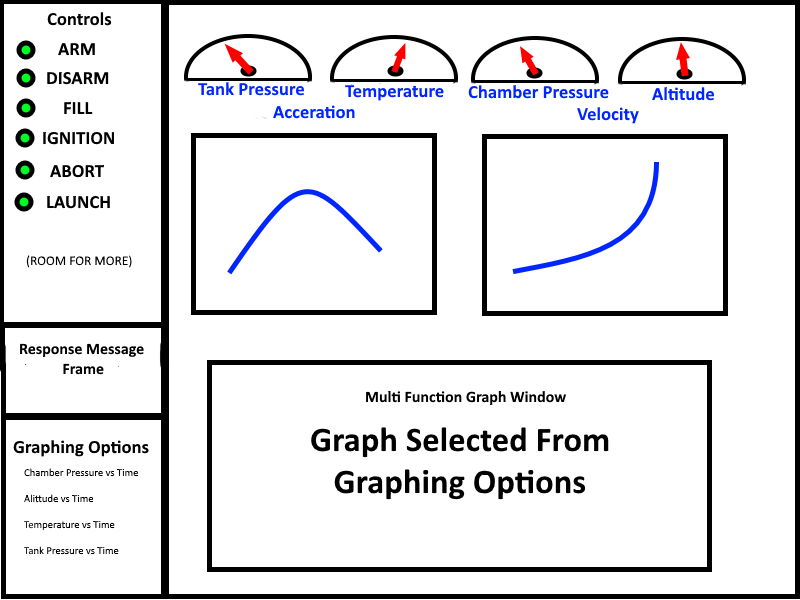
\includegraphics[scale=.85]{HyRoUIMockup}
\end{figure}

\subsection{The Command Buttons}
The command buttons are housed on the left side of the screen as depicted in the image above. These buttons will cause a command to be sent through the radio transceiver on the traditional computer to the radio transceiver on-board the rocket. The rocket will process the command and send a response back to be displayed in the message frame. The command buttons and their descriptions are as follows.\par

\begin{description}
\item[Fill] This will attempt to initiate the oxidizer fill process while the rocket is on the ground.
\item[Arm] This will adjust a servo prepare the rocket for ignition. Sequence number 2.
\item[Ignition] This will send a signal to igniter to ignite the rocket fuel. Sequence number 3.
\item[Launch] This will adjust a servo to release the rocket from its base. Sequence number 4.
\item[Disarm] This will adjust a servo to reverse the arming process. Can be used at any time.
\item[Abort] This will adjust all servos to their initial state. Can be used at any time.
\end{description}

\subsection{The Message Frame}
This is a small message box on the left hand side of the user interface directly under the command buttons. This box will display response message from the rocket. As message come in they will be appended to this message box. The box will be able to scroll if the messages exceeded the size of the frame.\par

\subsection{The Graphing Options Buttons}
These buttons are located on the left side of the user interface under the message frame. Each button will correspond to a specific graphing capability. When clicked on there will change which graph is displayed in the multi functional graphing window. Buttons and their corresponding graphs are listed below. \par

\begin{description}
\item[Chamber Pressure vs. Time] Clicking this button will change the multi function graph window to a graph of chamber pressure vs. time
\item[Altitude vs. Time] Clicking this button will change the multi function graph window to a graph of altitude vs. time.
\item[Tank Pressure vs. Time] Clicking this button will change the multi function graph window to a graph of tank pressure vs. time.
\item[Temperature vs. Time] Clicking this button will change the multi function graph window to a graph of temperature vs. time.

\end{description}

\subsection{The Gauges and Graphs}
Taking up most of the user interface on the right hand side are the gauges and graph canvases. Currently their will be 4 gauges that look like traditional gauges you would see on car dash board. They will be a semi circle with marks representing possible values of the data item. A arrow will be draw to represent the current value of the data. Below those gauges are two graphs representing velocity and acceleration these will graph these two data items vs time. Below the velocity and acceleration graphs is the multi function graphing window. This will display a user selected graph from the graphing options buttons selection menu. This will default to altitude vs time. Listed below are the gauges, graphs, and their units.

\subsubsection{Tank Pressure Gauge}
{\bf Units} \\ Tick marks are measured in pounds per square inch from 0 to 200.\par
{\bf Description} \\ This gauge represents the current pressure of the oxidizer tank. It will rise and fall along with the tank pressure. This value can also be graphed in the multifunction window.\par

\subsubsection{Temperature Gauge}
{\bf Units} \\ Tick marks are measured in degrees Fahrenheit from 32 to 300. 
{\bf Description} \\ This gauge represents the temperature wherever the temperature sensor is located. It will rise and fall along with the temperature surrounding the temperature sensor. This value can also be graphed in the multifunction window. \par

\subsubsection{Chamber Pressure Gauge}
{\bf Units} \\ Tick marks are measured in pounds per square inch from 0 to 200.\par
{\bf Description} \\ This gauge represents the pressure of the combustion chamber of the rocket. It will rise and fall along with the chamber pressure of the rocket. This value can also be graphed in the multifunction window. \par

\subsubsection{Altitude Gauge}
{\bf Units} \\ Tick marks are measured in feet above sea level from 0 to 10000.\par
{\bf Description} \\ This gauge represents the altitude of the rocket. It will rise and fall along with the altitude of the rocket. This value can also be graphed in the multifunction window. \par

\subsubsection{Acceleration Graph}
{\bf Units} \\ The x axis of the graph will be measured in meters per second squared and the y axis will be time from launch in seconds.\par
{\bf Description} \\ This graph represents the acceleration of the rocket with respect to time. The graph will be able to slide if the amount of data points exceeds the size of the graph window. \par

\subsubsection{Velocity Graph}
{\bf Units} \\ The x axis of the graph will be measured in meters per second and the y axis will be time from launch in seconds.\par
{\bf Description} \\ This graph represents the velocity of the rocket with respect to time. The graph will be able to slide if the amount of data points exceeds the size of the graph window. \par

\subsubsection{Multi Function Graph}
{\bf Units} \\ The x axis of the graph will be measured in different units depending on the graph chosen and the y axis will be time from launch in seconds.\par
{\bf Description} \\ This multi function graph will be the place where user selected graphing items are displayed. \par

\section{Bibliography}
\begin{thebibliography}{9}

\bibitem{BBB}
 BeagleBone.org,\\
\emph{(Tues November 29 2016)},\\
  \emph{Beagle Bone Black product information and website},\\
URL  http://beagleboard.org/black \\

\bibitem{ExampleSDD}
Unimap.edu example SDD,\\
\emph{(Tues November 29 2016)}, \\
  \emph{Unimap software development examples}, \\
URL http://portal.unimap.edu.my/portal/page/portal30/Lecturer\%20Notes/KEJURUTERAAN\_KOMPUTER/Semester\%202\%20Sidang\%20Akademik\%2020112012/EKT420\%20Software\%20Engineering/Example\%20of\%20Software\%20Design\%20Document(SDD)/EDDISS.pdf \\

\bibitem{IEE1016}
IEE 1016 Software Design Specifications,\\
\emph{(Tues November 29 2016)}, \\
  \emph{IEE 1016 Document availble on campus}, \\

\bibitem{TKinter}
Python.org wiki,\\
\emph{(Tues November 29 2016)}, \\
  \emph{Tkinter python wiki on python.org}, \\
URL https://wiki.python.org/moin/TkInter\\

\bibitem{Matplotlib}
Matplotlib.org,\\
\emph{(Tues November 29 2016)}, \\
  \emph{Matplotlib.org website documentation}, \\
URL http://matplotlib.org/

\end{thebibliography}
%\section{Index}
%\printindex
 
\newpage

\textbf{Students:}

\vspace{5mm}
 

\noindent \namesigdate{Jason Klindtworth} \hfill \namesigdate[6cm]{Josh Asher}
\vspace{5mm}

\noindent \namesigdate{Layne Nolli}
 \vspace{5mm}

\textbf{Client:}

\vspace{5mm}
 

\noindent \namesigdate{Nancy Squires}


\end{document}